\documentclass{article}
\usepackage{graphicx}
\usepackage[usenames,dvipsnames]{xcolor}
\usepackage{hyperref}
\hypersetup{
	%pagebackref=true,
	pdfcreator={LaTeX with abnTeX2},
	pdfkeywords={abnt}{latex}{abntex}{USPSC}{trabalho acadêmico}, 
	colorlinks=true,       		% false: boxed links; true: colored links
	linkcolor=blue,          	% color of internal links
	citecolor=blue,        		% color of links to bibliography
	filecolor=magenta,      		% color of file links
	urlcolor=blue,
	allbordercolors=black,
	bookmarksdepth=4
}
\usepackage[utf8]{inputenc}
\usepackage{tipa}
\newcommand{\ttt}[1] {
	\texttt{<#1>}}
\newcommand{\tttt}[1]{\texttt{#1}}
% \usepackage{fontspec}
% \usepackage[mathletters]{ucs}
% \newcommand{\ttt}[1] {
% 	\texttt{<#1>}}
% \newcommand{\tttt}[1]{\texttt{#1}}
\usepackage{subcaption}

\begin{document}
\title{Basic concepts and tools for the Toki Pona minimalist language:
Wordnet synsets; analysis, synthesis and syntax highlighting of texts}
% Anthropological computation
\author{Renato Fabbri\\
\texttt{renato.fabbri@gmail.com}\\
University of São Paulo,\\
Institute of Mathematical and Computer Sciences\\
São Carlos, SP, Brazil
}
\maketitle
\begin{abstract}
  A minimalist constructed language (conlang)
  is useful for experiments and is comfortable for making tools.
  The Toki Pona conlang is minimalist both in the vocabulary
  (only 14 letters, X phonemes, and 120 words + 4 synonyms)
  and in the $\approx10$ syntax rules.
  The language is useful for being a used and somewhat established
  minimalist conlang with at least hundreds of speakers.
  In this article, we describe current concepts and resources
  for Toki Pona,
  and make available Python scripted routines for
  analysis and synthesis of texts and the specification of syntax highlighting schemes.
  We focus on the analysis of the basic vocabulary,
  as corpus analyses were found in~\cite{corpus}.
  The synthesis is based on the basic sentence template,
  relates to context by keeping track of used words,
  and renders larger texts by using a fixed number of phonemes (e.g. for poems)
  and number of sentences, words and letters (e.g. for paragraphs).
  Syntax highlighting is performed in 24bit true colors, currently only
  with the Vim text editor.
  Word colors reflect morphosyntactic classes given in the official dictionary
  and different solutions to necessary and arbitrary choices are described and implemented.
  In summary, this text holds potentially novel conceptualizations about,
  and tools and results in analyzing, synthesizing or syntax highlighting the
  Toki Pona language.
  % subj (li), obj (e), prepositions, qualification (word concatenation), 
  % sent (la), particles, mi-sina, pi, punctuation is freestyle, pre-verb,
\end{abstract}
{\bf keywords:} Natural Language Processing, Textual synthesis, Syntax highlighting, Wordnet, Toki Pona

\section{Introduction}\label{intro}
Toki Pona is a minimalist conlang (constructed language)
with only 124 words (120 without the synonyms).
Therefore, the concepts are usually very general and different,
and, without context, the words are rarely related through
meronymy and hyponymy.
Such a linguistic setting is desired because of the simplicity
which entails easier e.g. learning and tool making.
Another reason why the minimalistic language design is compelling
is the study and harnessing of the strong and weak forms of
the Sapir-Whorf hypothesis (linguistic relativity),
i.e. that language influences or dictates ones thought
and world experience.
Accordingly, one uses a conlang as a thinking tool (or platform)
or to make experiments about the influence language has on
the thoughts of the `speaker' (also writer and reader).
Toki Pona is often described as a tool to meditate,
to simplify the thinking processes, and as a way to modify
the mood and impressions about the world.~\cite{tp1,tp2,tp3,tp4}
In~\cite{interview}, Sonja Lang (the creator of Toki Pona),
describes that she has seen the language been used successfuly
in the context of management, creation of texts, legal texts,
etc.

In this article, we present a conceptual overview of the language,
which is fit both to the newcomer and to the expert.
We also summarize
texts and software gadgets
for Toki Pona that
were developed by us and by other Toki Pona users.
Most importantly, the conceptual overview is considerably different
from what we found in the literature~\cite{pu,pije,memrise},
with emphasis on simplicity and flexibility,
and the software routines yield analyses, syntheses
and highlighting Toki Pona what was thought to be complementary
to the software currently available.

Next subsections hold a description of the general resources available,
a historical note, and some words about natural and constructed languages.
Section~\ref{basic} describes Toki Pona's phonology and syntax.
Section~\ref{hacks} presents the software routines we made available
and immediate results, such as listings and statistics of words,
poems and short stories, and coloring schemes.
Conclusions and further work are in Section~\ref{conc}.
Appendix~\ref{mytoki} holds considerations about my usage of Toki Pona,
with thoughts of rule breaking and potentially new conlangs.
Appendix~\ref{ftp} holds final words in Toki Pona.

% definition, historic, status (groups, speakers, etc).

\subsection{Resources on Toki Pona}
One might organize current resources for the Toki Pona
language in: references and learning material, corpus,
websites, interaction groups (here users talk a post texts and comments), and software gadgets.
The main references of the language are:
  the official book ``Toki Pona: The Language of Good'',
    authored by Sonja Lang, the creator of the language;
the online book ``o kama sona e toki pona!'',
from jan Pije~\cite{kama}.
For a more comprehensive view of the resources available
for the user, we suggest following the links 
from~\cite{wikiToki}.
Section~\cite{third} holds a summary of what we found in software
gadgets related to Toki Pona.

\subsection{Historical note}
Toki Pona was developed as an internal and personal language
by Sonja Lang~\cite{interview}.
It was released as a draft in 2001 and in 2007 some documents
reported it to have a few hundred speakers.
The English official book~\cite{lipu} was released only in 2014.
In 2016, a version of the official book was released in French.
Nowadays, one finds a number of texts about Toki Pona and written
in it, and uses of Toki Pona for artificial intelligence~\cite{roila}
and software tools~\cite{tptoll1,tptool2,tptool3},
in social platforms such as Facebook groups~\cite{fbtp,fbtpt},
microblogging~\cite{tokilili}, Telegram~\cite{telegram} and IRC~\cite{irc}.

\subsection{Natural and constructed and artificial languages}
A language one uses (or might use) to communicate by speaking
and writing is called `natural language'.
A `constructed language' is a natural language built by someone or
a group, such as Esperanto, Toki Pona, and Lojban.
An artificial language is a language yield by artificial agents,
such as in AI routines, and might be considered
within `cultural evolution' studies.
Formal languages are defined by tokens and rules to
operate them, they span from computer programming languages
to math and formal models for natural languages.
Lojban is a constructed language with the purpose of being
an artificial language because it is more axiomatic.

Constructed languages are in some traditions called artificial
languages, but creators most often prefer to use the term `standardized'
or 'planned' language with the argument that the conlang
is rooted on natural languages, and 'artificial' is misleading~\cite{conlanWikip}.
The preferred terms seem to be planned or constructed languages
or conlang.
The construction of languages is called glossopoeia.
Toki Pona is a conlang which might be classified
as engineered for experiments, meditation and philosophy;
and suitable for auxiliary international language and
as an artistic language. 
% taxonomy, vocabulary, ontology, terminology, 

% conlangs, natural langs, programming langs, Lojban as an
% intermediary
% non-verbal languages, musical corporal language, 
% non-verbal languages confront Sapir-Whorf hypothesis.


\section{Overview of the language}\label{basics}
This section describes very succinctly the formation of
words and sentences in the Toki Pona language.
It should enable a newcomer to grasp the essentials
of the language and the experienced to
acquire new insights.
Furthermore, it is a solid reference of the phonological and syntax
rules.

\subsection{Phonology}\label{phonology}
Words in Toki Pona are written using only 14 letters:
\begin{itemize}
  \item Vowels a (open), e (mid front), o (mid back), i (close front),
    u (close back).
  \item Consonants j, k, l, m, n, p, s, t, w:
    \begin{itemize}
      \item Nasal: m (labial), n (coronal).
      \item Plosive: p (labial), t (coronal), k (dorsal).
      \item Fricative: s (coronal).
      \item Approximant: w (labial), l (coronal), j (dorsal).
    \end{itemize}
\end{itemize}

There are standard guidelines for pronunciation,
but the language allows for considerable allophonic
variation.
For example, /p t k s l/ might be pronounced
[p t k s l] or [b d g z \textipa{\!R}].
Especially for poetry, one might consider
j and w to be vowels
(e.g. j as 'i' and w as 'u').

Syllables are of the form (C)V(N):
an optional consonant, a vowel and an optional nasal consonant.
Non word-initial syllables must follow the pattern CV(N).
The following sequences are forbidden: ji, wu, wo, ti, nm, nn.

\subsection{Syntax}\label{syntax}
\subsubsection{Fundamental notions}
As in other natural languages, 
colloquial Toki Pona might have
incomplete sentences and deviate from the
norm.
The basic structure of sentences is:
`subject' (Noun) li `predicate' (Verb) e `object' (Noun).
The li might be repeated to associate more than
one predicate to the subject.
The particle li is omitted if the subject is a simple mi (I or us)
or sina (you). A discussion about issues (problems)
yield by this rule
and how I deal with them is in Appendix~\ref{mytoki}.

The e might be repeated to associate more than
one object to a predicate.
Sentences might be related though la,
'sentence' la 'sentence', where the second sentence is
the main sentence, and the first sentence is a condition
to the first.
Multiple la-s are not described in literature,
but I assume that one might assume the last sentence
being a conditional to the next,
except in cases where the context strongly suggests
otherwise.

Noun and verb phrases are (usually) built with the non-particle words.
The first word is the noun or verb and subsequent words
qualify the noun or verb.
The pi particle might be used to separate sequences of words
to be evaluated before the relation yield by pi.
As pi is often ill understood and used,
the following structures might be handy for newbies and as a
reference:
\begin{itemize}
  \item No pi, `word word word':
word $\leftarrow$ (qualifies 1) word $\leftarrow$ (qualifies 2)  word.
  \item One pi, 'word pi word word': word $\leftarrow$ (qualifies 2) [
      word $\leftarrow$ (qualifies 1)  word ].
  \item Two pi-s: `word pi word word word pi word word':
    word $\leftarrow$5 [word 2 word] 3 word $\leftarrow$4 word 1  word;
or:
    word $\leftarrow$5 [word 1 word] 2 word $\leftarrow$4 word 3  word.
\end{itemize}

Notes on the usage of pi:
\begin{itemize}
  \item In a sequence of words, without pi, the second word qualifies
    the first, the third word qualifies the phrase yield by the first
    two words, the fourth word qualifies the noun yield by the first
    three words and so on.
  \item It is redundant to use pi before the last word in a noun or
    verb phrase if there is no other pi, reason why it is most often
    omitted.
    Its use in this case is regarded as wrong~\cite{lipu,pije},
    but, as one might notice, it does not add (much) information
    through syntax (order of qualifies is conserved).
    It adds as an emphasis because of greater length of the written segment, as a preparation: 'jan lili pi mama' (mommy's child).
    Also used in~\cite{akesiWawa}.
  \item The book by jan Pije~\cite{kama} describes another use for pi:
    after li to mean possession, e.g. `soweli li pi sina' (your pet).
    This employment of pi might be regarded as correct, but are promptly written
    as a noun phrase (e.g. `soweli sina') and is not mentioned
    by the official book~\cite{tpLabg}.
\end{itemize}

All the words except the structural particles (li, e, la, pi)
are usable in any position in noun and verb phrases,
(i.e. 116 words).
Notice that the phrase expresses a noun in a noun phrase (subject or
object) or a verb (in the predicate).
And that the first word of the phrase is the noun or verb,
and that subsequent words are adjectives or adverbs.
The pi and other particles restarts the phrase to
first word being a noun.

At this point, the only missing syntax rule is related to
the prepositions: kepeken, lon, sama, tan, tawa.
They might appear at the end of phrases,
should be followed by another phrase,
and require no particle. E.g.
`toki *tan* jan Pije li pana e sona *tawa* mi'.
Because prepositions can be used as adjectives
or nouns or verbs, adverbs, etc, and what follows
a preposition complement might also be of any morphosyntactic class,
they are core sources of ambiguity.
three:
* preposition
* absence of li on sina and mi
* Incomplete sentences
(ona li) tawa lon kon e ilo pi suli mute

\subsubsection{Particles}
Beyond the structural particles (li, e, la, pi) presented
in last section, other particles are:

\begin{itemize}
  \item a or kin, emphasis.
  \item o, vocative or imperative ('jan lukin sitelen o, li wawa')
  \item taso, means however as sentence or 'only' if adjective.
  \item anu, en: 'or' and 'and'. Used for nouns in nous phrases.
    For repetition of verbs, repeat li.
    For object nouns, repeat e.
    If the noun is complementing a preposition (tawa, lon),
    one might repeat the preposition.
    As Toki Pona is a recent language, and is able to cope with
    variation due to its simplicity, I would advocate for
    using en and anu wherever there is no ambiguity.
    E.g.: 'mi tawa anu moku lon tenpo lili?'
    In the official documentation that is not described and
    might be regarded as wrong in strict canonical.
  \item nanpa, denotes numbering.
  \item seme, for questions, used next to the thing being asked for.
    'Why?' might be expressed as
    'seme la sina pana e moku lon sewi'.
  \item mu, for animal noises. For me it is not a particle, as in the
    official dictionary, but a noun.
    I also like to use it as a verb:
    'mi pakala e luka. mu mute.'
\end{itemize}

The vocabulary specifies morphosyntactic classes:
nouns, adjectives, verbs, pre-verbs, adverbs, particles, prepositions, and numbers.
I find that they might help the user and newcomer, but
it might also suggest a deviation from what I understand and read:
the words might be used indistinctly to be the nouns
(subjects, the predicate when there is no object, objects,
and preposition complements),
the adjectives (anything that does not start the noun phrase or follows a pi),
verbs
(follows mi or sina or li or a preposition),
adverbs (follows the verb).
The pre-verbs (wile, ken, awen, kama, lukin, sona),
might follow a verb, but might also be understood
as the verb qualified with the next word,
which carries a very similar if not identical meaning.
The pre-verbs are all also defined as other morphosyntactic classes,
such as adjective, noun, verb.
The only exception is wile, which is only a pre-verb.

Thus, the classes given in the dictionary dictate little
in practice:
jan kala li lape lon ni.
Where kala, lape and ni are in this phrase
as adjective, verb and noun,
and are in the dictionary as noun,
adjective and adjective.

As far as I can see, one should regard
the particles li, e, pi, and la
and punctuation.
The other tokens of the vocabulary
might be used in any of the remaining positions.

\subsubsection{Convention for recognizing POS tags by speaker and machine}

\begin{itemize}
  \item Noun: the first word in a noun phrase.
    After an 'e' and after a pi,
    The first word in the sentence if
    sentence does not start by the verb.
    Might be in the position of the verb
    if the sentence has no object.
  \item Adjective: second word on after an e and after
    Second word on in the subject phrase if present.
  \item Verb: after a li, mi or sina.
    If there is no object, the verb position
    is often a noun.
  \item After a preposition,
    there can be a noun phrase, a verb phrase
    or nothing.
  \item Notice that there is ambiguity in the structure
    introduced by the omission of li after mi and sina.
    Also, when there is no object, a noun or a verb
    or an adjective might be in the verb position
    if there is no object.
    The prepositional complement is also not defined.
    (mi moku tawa pali, tawa tomo).
    So, these are sources of syntactic ambiguities
    in Toki Pona.
    They might be solved or minimized by using the semantics
    of the words.
    One preliminary effort in this direction might be
    using the classes in the official dictionary to resolve
    ambiguities whenever possible.
    This solution is not optimal in correct POS tagging,
    and does not solve all possible ambiguities
    (there are words classified as nouns and adjectives,
    adjectives and verbs, nouns and verbs, particle and verb).

    Another source of ambiguity is the pre-verbs as described
    in the literature~\cite{tpLang,pije}.
    But I find it reasonable to understand them as verbs.

\end{itemize}

Also, the prepositional complement might
be a noun or a verb.
I could not come up with a sentence
where it would be understood as an adjective.


\subsubsection{Further notes}
The only synonyms on Toki Pona are:
a and kin; lukin and oko;
sin or kamako;
ale or ali.

In formations such as
toki e ni:, wile e ni:, tan ni: etc.
'(e) ni' can be omitted and : used alone.

Names are by default transliterated,
but might not be, as described in Section~\ref{mytoki}.


% my view
% considerations about the official book and jan Pije
% pictorial forms
\section{Software for analysis, synthesis, and syntax highlighting}\label{hacks}
In this section,
we describe software, natural language, audiovisual and numeric results
on four directions:
1)
the analysis of the Toki Pona language through statistics
obtained by processing the dictionary;
2)
the synthesis of sentences, poems and short stories
in Toki Pona;
3)
syntax highlighting for Toki Pona,
including fine-tuning and theoretical
considerations;
4)
initial considerations about the WordNet of
Toki Pona words.
Corpus analysis was already found in~\cite{}.

The Python scripts (or the toolbox)
for obtaining all the results in this sections,
and more, is publicly available in~\cite{tokipona},
to facilitate both the inspection of the results and the
generation of derivatives by other interested parties.


\subsection{Statistics of the vocabulary}\label{sec:stat}
In~\cite{pije} are statistics about Toki Pona corpus.
This section focuses on the statistics of the vocabulary
and syntactic rules:
the letters, phonemes, word sizes,
possible combinations for words and sentences.
The statistics are in Appendix~\cite{listings},
and the next paragraph is an overview.
The script \tttt{makeStatistics.py}
was used to obtain the all the measurements and tables
discussed herein,
and hold some other measurements and sets of words
which were regarded as less suitable for this exposition.

As described in Section~\cite{basics},
there are only 14 letters,
and phonemes respect a few rules.
There are 120 different words in the official vocabulary,
4 of them having synonyms.
A total of 124 tokens,
not counting proper nouns (names)
and punctuation.
Table~\ref{tab:pos} shows the number of words
related to each POS tag specified in the dictionary.

\begin{table*}[h!]
\begin{center}
\caption{POS tags incident and chosen.
            The official dictionary often relates one token
            to more than one POS tag.
            For the current version of the text highlighting plugin described in
            Section~\ref{shigh}, for example,
            a token needs to have an established tag to have
            a defined color.
            On the 'Chosen' column, the tokens were regarded only once
            by choosing the class in the dictionary respecting the
            precedence order: PRE-VERB, VERB, PREPOSITION, PARTICLE, ADJECTIVE, NOUN, NUMBER.}\label{foobar}
\begin{tabular}{ l | c c }
POS & All  & Chosen \\\hline
NOUN & 58  & 49 \\
ADJECTIVE & 40  & 34 \\
VERB & 15  & 13 \\
PARTICLE & 12  & 12 \\
PRE-VERB & 6  & 6 \\
PREPOSITION & 5  & 5 \\
NUMBER & 4  & 1 \\\hline
total & 140  & 120 \\
\end{tabular}\end{center}
\end{table*}


From the official 124 words, 
26 of them (20.97\%)
have only one syllable,
85 (68.55\%) have two syllables,
and 13 (10.48\%) have three syllables.
No official words has four or more syllables.
Of all the 235 syllables of the official words,
li, la, ka, na, and pa are the most often (with 5.53\%,
4.26\%, 3.83\%,  3.83\%, 3.83\%).
On the first syllable of each word,
a, o, pi, ka, and la are the most often
(with 6.45\%, 4.03\%, 4.03\%, 3.23\%, 3.23\%).
On the last syllable of each word,
li, lo, na, la, and ma are the most often
(with 8.06\%, 4.84\%, 4.84\%, 4.03\%, 4.03\%).
Middle-word syllables only occur 13 times,
and are all different, with the exception of `la',
which occurs twice.
For the frequencies of all syllables in every position,
run the script \tttt{makeStatistics.py} in~\cite{tokipona}.

Vowel and consonant frequencies are as shown in Table~\ref{freqLet}
for starting, end and internal position.
Comparison of vowels against consonant is in Table~\ref{tab:vcon}.
The high incidences e.g. of 'l' and 'a' favor
the naturalness of the language prosody
as it resembles child speech.

\begin{table*}[h!]
\scriptsize
\begin{center}
\caption{Frequency of letters in Toki Pona.
            freq, freq\_I, freq\_L and freq\_M are
            the frequencies of the letters in any, initial, last and middle
            positions.
            The columns 'v' and 'c' that follow them are frequencies
            considering only vowels and consonants.
            The most frequent vowel is 'a' in any position,
            although it is more salient among words starting with a vowel
            and among the last letter of the words.
            For starting, ending and middle positions, the second most frequent
            vowel varies.
            Among the consonants, 'n' is the most frequent because it is
            the only consonant allowed in the last position and because
            almost 20\% of the words end with 'n'.
            On the initial position, 's' is the most frequent consonant,
            while in middle position 'l' is the most frequent consonant.
            Many other conclusions can be drawn from this table and are
            useful e.g. for exploring sonorities in poems.}\label{freqLet}
\begin{tabular}{  l | c   c   c | c   c   c | c   c   c | c   c   c  }
letter & freq  & v  & c  & freq\_I  & v  & c  & freq\_L  & v  & c  & freq\_M  & v  & c \\\hline
a & 16.35  & 33.19  & -  & 8.06  & 40.00  & -  & 29.03  & 35.64  & -  & 14.22  & 29.46  & - \\
e & 8.60  & 17.45  & -  & 2.42  & 12.00  & -  & 11.29  & 13.86  & -  & 10.78  & 22.32  & - \\
i & 11.53  & 23.40  & -  & 3.23  & 16.00  & -  & 20.97  & 25.74  & -  & 10.78  & 22.32  & - \\
o & 7.55  & 15.32  & -  & 4.03  & 20.00  & -  & 14.52  & 17.82  & -  & 6.03  & 12.50  & - \\
u & 5.24  & 10.64  & -  & 2.42  & 12.00  & -  & 5.65  & 6.93  & -  & 6.47  & 13.39  & - \\\hline
j & 2.10  & -  & 4.13  & 3.23  & -  & 4.04  & 0.00  & -  & 0.00  & 2.59  & -  & 5.00 \\
k & 6.29  & -  & 12.40  & 11.29  & -  & 14.14  & 0.00  & -  & 0.00  & 6.90  & -  & 13.33 \\
l & 9.22  & -  & 18.18  & 12.10  & -  & 15.15  & 0.00  & -  & 0.00  & 12.50  & -  & 24.17 \\\hline
m & 4.61  & -  & 9.09  & 10.48  & -  & 13.13  & 0.00  & -  & 0.00  & 3.88  & -  & 7.50 \\
n & 10.48  & -  & 20.66  & 6.45  & -  & 8.08  & 18.55  & -  & 100.00  & 8.19  & -  & 15.83 \\
p & 5.66  & -  & 11.16  & 11.29  & -  & 14.14  & 0.00  & -  & 0.00  & 5.60  & -  & 10.83 \\\hline
s & 6.29  & -  & 12.40  & 13.71  & -  & 17.17  & 0.00  & -  & 0.00  & 5.60  & -  & 10.83 \\
t & 3.14  & -  & 6.20  & 6.45  & -  & 8.08  & 0.00  & -  & 0.00  & 3.02  & -  & 5.83 \\
w & 2.94  & -  & 5.79  & 4.84  & -  & 6.06  & 0.00  & -  & 0.00  & 3.45  & -  & 6.67 \\
\end{tabular}\end{center}
\end{table*}

26, 85 and 13 words have one, two and three syllables
(20.96, 68.54 and 10.48\% of all 124 tokens).
No official word have more than three syllables
(although proper names may be of any size).
In all the 124 tokens, there are 235 syllables (68 different).
Most often syllables are in
Table~\ref{syl}.
A complete list of the syllables and their frequencies (in different
positions) is in the \tttt{hsyls} variable of the \tttt{makeStatistics.py}
script.
A list of all words, grouped by their size in syllables,
and ordered alphabetically and by the number of letters,
is in \tttt{hlsyl\_\_}.

\begin{table*}[h!]
\begin{center}
\caption{Frequency of syllables in Toki Pona
            considering all 235 syllables of the 124 tokens,
            only the first or last syllables or only the middle
            syllables.
            In parenthesis are the count and percentage of the
            corresponding syllable. For more information and a
            complete list of syllables, see Section~\ref{sec:stat}.
            }\label{tab:freqSyl}
\begin{tabular}{  l | c   c   c   c  }
rank & all  & first  & last  & middle \\\hline
1 & li (13, 5.53\%)  & a (8, 6.45\%)  & li (10, 8.06\%)  & la (2, 15.38\%) \\
2 & la (10, 4.26\%)  & o (5, 4.03\%)  & lo (6, 4.84\%)  & je (1, 7.69\%) \\
3 & ka (9, 3.83\%)  & pi (5, 4.03\%)  & na (6, 4.84\%)  & ka (1, 7.69\%) \\
4 & na (9, 3.83\%)  & ka (4, 3.23\%)  & la (5, 4.03\%)  & ke (1, 7.69\%) \\
5 & pa (9, 3.83\%)  & la (4, 3.23\%)  & ma (5, 4.03\%)  & li (1, 7.69\%) \\
6 & a (8, 3.40\%)  & pa (4, 3.23\%)  & pa (5, 4.03\%)  & lu (1, 7.69\%) \\
7 & ma (8, 3.40\%)  & se (4, 3.23\%)  & ka (4, 3.23\%)  & ma (1, 7.69\%) \\
8 & si (8, 3.40\%)  & si (4, 3.23\%)  & sa (4, 3.23\%)  & me (1, 7.69\%) \\
9 & lo (7, 2.98\%)  & su (4, 3.23\%)  & si (4, 3.23\%)  & pe (1, 7.69\%) \\
10 & pi (6, 2.55\%)  & i (3, 2.42\%)  & te (4, 3.23\%)  & ta (1, 7.69\%) \\
\end{tabular}\end{center}
\end{table*}


Given the rules given in Section~\ref{phonology}
(of 14 letters, 5 vowels, (C)V(N) phonemes,
forbidden ji, wu, wo, ti, nn, nm),
96 words are possible with 1 syllable,
8256 with 2 syllables, 710016 with 3 syllables.
No middle syllable end with the nasal consonant 'n'.

Possible syntactic structures are unlimited.
For a noun or verb phrase, one might quantify the possibilities
by considering all words but the particles that are nothing else
(i.e. li, e, la, pi, a, o, anu, en, seme, mu)
and the presotions that are nothing else (i.e. kepeken, lon, tan).
This yields $120-13=107 words$.
As discussed in Section~\ref{syntax},
I advocate that, although such words are classified in the dictionary,
they might be used indistinctly as nouns, adjectives,
verbs and adverbs.
Thus, one have 107 possibilities of noun and verb phrases with
one word, $107^2=11449$ possibilities with two words,
$107^3=1225043$ with three words and so on.
Be $n$, $v$, $o$, and $p$ the number of words in the subject (noun), predicate
(verb), object (noun) and prepositional (noun or verb) phrases of a sentence,
and assume that the sentence has at most one prepositional phrase,
one might quantify the possibilities using the formula:
$\delta = 107^n\times 107^v\times 10^o \times 5\times 107^p$,
where $5$ stands for the possible prepositions.
To account for the particles, one possibility is
to assume for simplicity that one might use none or one particle
(not li, e, la, pi, resulting in $8$ particles and $9$ possibilities)
at each phrase, yielding:
$\delta = 107^n\times 107^v\times 107^o \times 5\times 107^p\times 9^4$.
For example, assume $n=v=o=p=1$, then
$\delta=107^1\times 107^1\times 107^1 \times 5\times 107^1\times 9^4=
 4.300066\times 10^+12$
i.e. more then 4 trillion possible
sentences with single word phrases (i.e. no adjectives or adverbs),
while allowing only one particle per phrase
and only one predicate phrase 
(e.g. 'ona li moku e soweli lon supa').
The general case is implemented as a function
in the script \tttt{makeStatistics.py}~\cite{tokipona}

\subsection{Synthesis of text}\label{synth}
Such counting exercises are also useful
for facilitating (semi-)automated writing through scripting.
The syntax organizes the words in larger structures.
The rhymes are restricted and sonorities are
restricted by the small vocabulary and simple syntax.
There are some specific tasks for achieving texts,
such as finding the number of syllables considering the elisions,
or handling interaction of the writer with the script
to choose sentences or verses or stanzas.

\begin{figure}     \center
  \begin{subfigure}{.5\textwidth}
    \centering
        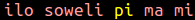
\includegraphics[width=.8\linewidth]{figs/phrase_}\vspace{-0.15cm}
          \caption{Synthesized phrase.}
            \label{fig:sfig1}
  \end{subfigure}\\\vspace{0.3cm}
  \begin{subfigure}{.9\textwidth}
    \centering
        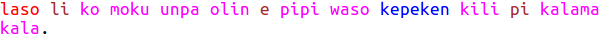
\includegraphics[width=1.2\linewidth]{figs/sentence_}\vspace{-0.15cm}
          \caption{Synthesized sentence.}
            \label{fig:sfig2}
  \end{subfigure}\\\vspace{0.3cm}
  \begin{subfigure}{.8\textwidth}
    \centering
        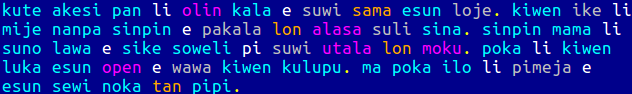
\includegraphics[width=1.2\linewidth]{figs/paragraph_}\vspace{-0.15cm}
          \caption{Synthesized paragraph.}
            \label{fig:sfig2}
  \end{subfigure}\\\vspace{0.3cm}
  \begin{subfigure}{.7\textwidth}
    \centering
        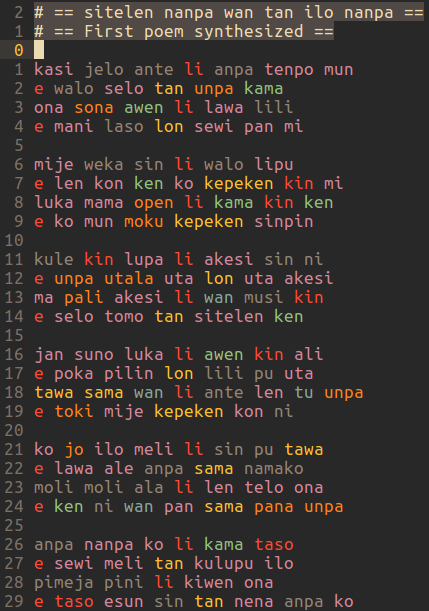
\includegraphics[width=.8\linewidth]{figs/poem_}\vspace{-0.15cm}
          \caption{Synthesized poem.}
            \label{fig:sfig2}
  \end{subfigure}
  \caption{Toki Pona texts synthesized by the scripts
  in~\cite{tokipona}: (a) a phrase, (b) a sentence, (c) a paragraph,
  and (d) a poem.
  The unusual formations are convenient for exploring semantic
  possibilities.
  A user might obtain many of such structures to select those
  he/she finds fit for the intended employment.
  For more information, see Section~\ref{synth}.
  The words are colored in accordance to the considerations
  of Section~\ref{shigh}.}
  \label{fig:syn}
\end{figure}


The same package~\cite{tokipona}
has capabilities for synthesizing Toki Pona text.
On its most basic level, the routines yield
noun, verb and prepositional phrases,
sentences.
They also aim at making larger scale texts
by keeping a record of the used words and structures (context)
and using stylistic outlines for poems and short narratives.

Figure~\ref{fig:syn} holds some synthesized texts
with different coloring schemes for syntax highlighting,
as presented in the next section.
The textual synthesis described here,
and implemented in \tttt{makeTexts.py}
might be enhanced as described in Section~\ref{conc}.

Automatic and randomized synthesis of texts in Toki Pona are
useful because of the reduced vocabulary: ideas often make
sense in unexpected way, and yield a way to 
explore the semantic field possible by Toki Pona.
Each words is related to a broad semantic field,
thus the randomized selection of words are more likely
to make sense.
One might object that the resulting texts are unusual 
and even consider that they often hold insubstantial or unsound meaning.
We advocate that these unexpected formations are desirable
for exploring the possibilities of the language and of thought,
and for artistic endeavors.
Also, to obtain texts which one finds usual or satisfactory
in more strict or personal terms, such a person might just write
them normally.

% phrase
% sentence
% poem
% text
% each with a different color scheme

% nanpa followed by numbers
% pu, taso, kin/namako
% particles
% rhymes 
% modes in which the words are only used as specified in the dictionary

\clearpage
\subsection{Syntax highlighting}\label{shigh}
The same package~\cite{tokipona}
has a Vim~\cite{vim} syntax highlighting plugin
for Toki Pona,
routines to arrange the coloring schemes
(i.e. to yield the text files with the specifications for which tokens
to relate to which coloring groups),
and instructions for installing and using
the resulting syntax highlighting for Toki Pona texts~\cite{tokipona}.

Basically, it distinguishes the words among the morphosyntactic
classes according to the official dictionary as given in
Table~\ref{foobar}.
A word often belongs to more than one class,
thus the precedence of them might be set by the user.
Also, some classes might be further refined (e.g. words beginning with
vowels) or joined (e.g. distinguishing only particles and the rest,
or particles and prepositions and the rest).
The colors are also promptly changed according to~\cite{vimArt}
and exemplified in the package documentation.

Currently, the Python package synthesizes the
syntax file through the\\ \tttt{makeVimSyntax.py} script.
The user has control of class precedence and
merging and further details through tweaking such routine.
The choice of precise coloring schemes
involves fine tuning the color scheme being
used in Vim (such as 'blue', 'elflord' and 'gruvbox'),
and Vim's highlighting schemes as described in~\cite{vimArt}.
In summary,
the usage of the package and plugin might be performed
through the following actions:
\begin{itemize}
  \item Installation of the plugin.
  \item Tweaking of the syntax file by hand.
  \item Running the \tttt{makeVimSyntax.py}
    Python script to generate a new syntax file
    according to other settings.
  \item Write a file names with the \tttt{.tokipona} or \tttt{.tp} extension
    (inside Vim) using Toki Pona words.
    Reload the highlighting scheme using \tttt{:e} whenever you
    change the syntax file by hand or through the Python script.
  \item Access the used highlighted groups with :syntax,
    Access all the highlighting groups with \tttt{:so
    \$VIMRUNTIME/syntax/hitest.vim} or \tttt{:hi}.
    Change the coloring of a set of terms by associating
    a used group (e.g. tokiponaADJECTIVE) to an existing group (e.g.
    Visual) such as in \tttt{:highlight link tokiponaADJECTIVE Visual}.
\end{itemize}

The tokipona.vim syntax file has an association of toki pona
words with highlighting groups.
It also holds association of these groups to other groups
to use their color settings.
Therefore, one is able to use various color schemes
with syntax-highlighted Toki Pona texts.
A Vim user might run e.g. \tttt{:colorscheme blue},
\tttt{:colorscheme solarize}, \tttt{:colorscheme gruvbox} or
\tttt{:colorscheme elflord} to see the same text colored
with different color schemes (association of colors to sets of tokens).
To interfere directly on the colors chosen,
\tttt{:highlight Normal guifg=\#00000 guibg=\#0000ff}
will change the standard foreground (text) color to pure black
and background to pure blue.
See \tttt{:h gui-colors} and \tttt{:h highlight}
for the way you might edit colors directly.
Useful commands are given as commented lines
in the end of the syntax file.
One might obtain an HTML file with the colored Toki Pona text
by using the \tttt{:TOhtml} command.

% reference to figure of the texts.

\subsubsection{Advanced syntax highlighting considerations}
Standard guidelines for syntax highlighting
depend heavily on cultural and use factors
and have scarce scientific studies~\cite{stack}.
There are informed projects such as Solarized~\cite{solazired},
which present solutions for some contexts.
Strikingly, standard guidelines for syntax highlighting were not found.
Therefore, we considered current data visualization
theory~\cite{dv1,dv2,dv3,dv4} to glimpse at the potential guidelines:
\begin{itemize}
  \item The use of blue and other high frequency colors for
  background.
  This is extended to other high frequency (small wavelength)
  colors such as violet.
  \item The avoidance of blue and other high frequency
  colors to fill small objects, such as letters and words.
  \item Explore simplicity and elegance through the use of discrete
  coloring schemes. Most of the tokens should be preferably of
  the same color.
  One might use a power-law to mimic natural occurring phenomena.

  Unfortunately, the dictionary classification of words are not in a
    power-law distribution and might be better described by a half-normal or by
overlapping normal distributions over the three peaks ($\sim35-58,
12-18, 1-5 occurrences$).
  \item Physical stimuli might be related to perceptual stimuli both 
    through a power-law or an exponential law (respectively known
    as Steven's law and Weber-Fechner's law).
  \item One usually wishes to maximize contrast,
  although taste and less wearing combinations might
  also dictate the coloring choices.
  \item Stipulate axes of parameters with which to set colors.
  Wavelength or frequency is an obvious axis given the considerations
  above.
  Other parameters are hue, transparency etc.
  \item One might consider two types of color schemes: those with a dark background,
  which are more comfortable at first; and those with a light background,
  which are usually impressive (and even annoying) at first,
  but the eye gets used to it and it keeps you more stimulated.
\item The blue color is specially related to physiological
  stimulation of the body~\cite{blue,blue2},
    and programmers often report that a blue background keeps them
    awake and more concentrated.
    I found no evidence of this in the scientific literature,
    and one might simply take my word that programmers say so
    since I now have programmed daily for more than 10 years.
  \item Consider that the user might stay many hours (and we often do)
  at a text editor, and that the colors and formats involved are
  prone to entail a considerable effect in the body and mental
  activity and thus in the quality of life and work of a programmer.
  \item Syntax sonification: consider mapping the textual structures
  to sound (i.e. parametrize the synthesis of sounds e.g. 
    by the counting of specific tokens inside a script, a function or
    class or around a variable of conditional or
    loop)~\cite{mass}.
  \item Ideally, one should have facilities for tuning 
    the syntax highlighting (e.g. through keyboard shortcuts)
  as envisioned in~\cite{vimArt}.
\end{itemize}

On the consideration of writing and of Toki Pona,
the considerable irrelevance of the morphsyntactic classes as
described in Section~\ref{} suggest that a appropriate coloring should
consider the syntax to identify the nouns, verbs, adjectives, adverbs,
prepositions and particles.
Also, the coloring for poems might be more appealing if considered
e.g. the counting of syllables or repeated vowels and ending
syllables.
Insights might be obtained through the observation of the
choices made and advocated in software packages such as text editors
(e.g. Vim, Emacs, Sublime, etc.),
software dedicated to syntax highlighting (e.g.
pigments \footnote{\url{http://pygments.org/docs/}} and 
highlight.js \footnote{\url{https://highlightjs.org/}},
other software (e.g. Linux terminals such as Xterm and gnome-terminal).
Finally, the careful choice of fonts is known to have
a relevant impact in comfort and productivity~\cite{fonts},
e.g. sans-sheriff fonts are more promptly read and yield a cleaner
text than a for with sheriff.

\subsection{Wordnet Toki Pona}\label{wn}
For the achievement of a first Toki Pona Wordnet,
each of the Toki Pona words in the dictionary
were related to Wordnet synsets
through the English lemmas.
All synsets related to the lemma with the POS tag
given in the dictionary are added.
Another immediate possibility would be to
relate each Toki Pona word to the synsets
simultaneously associated to all the English
words bounded by a semicolon in the dictionary.
Yet another possibility, which I find more consistent
but also more controversial,
is to choose all synsets related to the English
words given that the Toki Pona words can be used
in many roles.
Wordnet only contains nouns, adjectives, verbs, and adverbs.
Thus, particles and prepositions were not considered.
Numbers were considered adjectives.
Words presented as adjectives in the dictionary
were considered adjectives and adverbs.~\cite{wordnet}

The total number of different synsets is $2493$ in a very conservative
counting: discarding prepositions and particles,
and only considering the synsets which have the POS tag
given in the dictionary.
If all the synsets (that have any POS tag)
related to a lemma are considered, 
then Toki Pona vocabulary reaches $3961$ synsets.
The prepositions are particularly missing in such
countings because e.g. tawa or lon are used also
as ordinary words.
If synsets for them are considered those of the English
lemmas with any POS tag, the vocabulary reaches $4052$
synsets.
The total number of synsets in Wordnet is $117659$.
Total number of synsets counting neighbors is Y.
Depth of TP synsets is .
We envision the usage of such features to guide creation
of other conlangs.

The \tttt{makeWordnet.py} script, available in~\cite{tokipona},
makes available such a tentative Wordnet in the simplest form:
the Toki Pona words are keys in a dictionary that returns the
corresponding synsets.
Three of such dictionaries are implemented:
one where all synsets related to the lemma is
returned; another as such but excluding the prepositions;
one that returns only the synsets
registered in Wordnet with the same POS tag as the lemma
is in the official dictionary. 

It is worth mentioning that Toki Pona words are very general
and each of them might mean many things.
Thus, the words are not very easily related e.g. by hyponymy
or meronymy.
Exceptions: jan (people) is a hyponym of soweli (mammal);
kili is an hyponym of kasi;
walo, pimeja, jelo, loje, laso
are hyponyms of kule;
luka (as hand) is a meronym of sijelo (as body).

\subsection{Hacks and resources from other people}
A number of tools and other resources for dealing with Toki Pona
were developed by the community.
The most complete list is supposedly~\cite{gdoc} and includes
videos, musical pieces, artistic texts, reference documents (e.g.
a Toki Pona - Esperanto dictionary), journalistic articles,
and software tools.

\section{Conclusions and further work}\label{conc}
\begin{itemize}
  \item Further develop the text synthesis facilities described in
    Section~\ref{synth} might be enhanced by further employing e.g.
    rhythm, meter, rhyme and form techniques~\cite{wikipPoetry}.
  \item Make a syntax highlighting that colors the tokens with respect
    to the syntatic position and function, and not in a fixed manner
    as is implemented and exposed in Section~\ref{shigh}.
  \item Relate Toki Pona to Wordnet: should one Toki Pona word
    be related to more then one synset of the English language?
    An immediate implementation would be linking each Toki Pona word
    to the English words in the official vocabulary.
    A Toki Pona synset would be related to all the synsets of each English
    words regarded as lemmas (sequence of characters or sound).
  \item Translators. This Toki Pona Wordnet would be useful e.g. for naive translators
    of words and text.
    Enhancements of such translators would use POS tagging and templates
    in English and Toki Pona and/or corpus and further statistical methods.
    An efficiency of Toki Pona can be studied in terms of the coverage of
    the Wordnet cloud.
  \item Conlanging. In fact, I plan to use Wordnet for making new conlangs
    (conlanging), and insights derived from Toki Pona might be used for that end.
  \item Understand how the corpus is gathered in \url{tokipona.net}.
  \item Know about previously existing words that were used for Toki Pona
    (e.g. suno and suwi might come from sun and sweet),
    and about the reasons that lead Sonja (and maybe other people)
    to choose the 14 letters and the syllable structure.
    This might require a dedicated communication with the
    speaker community and the documentation authors.
  \item Corpus-based analysis.
  \item Publication of original texts and translations.
  \item Make an article written in Toki Pona.
    I wrote Section~\ref{finalToki}, and believe that
    a summary in both English and Toki Pona for
    facilitating the acquisition of context,
    a reasonable article on some scientific topics is
    possible.
    I first conceived something around complexity, statistics, physics, or computer science.
    But one possibility is to write about linguistics, philosophy, literature
    or psychology with the partners I write in English.
    I can start a draft,
    qhey might learn the language in a few hours (with or without my help),
    to contribute, and we can write a short paper.
  \item Enhance the synthesis of text to yield better contextualized text
    and stylistic traces, such as for poems and short stories.
    Give the user the ability to choose the sentences (generate randomly according to
    previously written or given text,
    some rules input by the user, the package and the language guidelines,
    outputs to the screen and asks to keep and discard).
  \item Enhance the syntax highlighting implementation described in Section~\ref{high}.
    It uses only syntactic cues to choose POS tags,
    which might be overcome by using n-grams and
    further techniques from Natural Language Processing~\cite{POS}.
  \item We are particularly interested in software tools,
    and one possibility is to use a conlang to describe software
    routines.
    In this sense, it seems profitable
    to understand what `non-ambiguous' means in Lojban,
    and in what sense one is able to compile and parse Lojban.
    This study will probably yield considerations about
    parsing Toki Pona files.
  \item Conlang idealized for describing data, programs,
    scientific writings, creative writing
    (exploring the thinking process).
    Different modes that might be specified by a section header or tag.
  \item The plugin comes with the :TokiStation command, which opens a window with the files: ijositelen.tokipona, makevimSyntax.py, Highlight Test (created by hitest.vim above), syntax/tokipona.vim.  Another tab with shells: python to run over the makeVimSyntax.py and make new syntax/tokipona.vim files. Another with Readme, and PDF documentation. Another with an IPython. Imported tokipona. It resets completely upon command :TokiClose, closing all created windows.
\end{itemize}

\subsection*{Acknowledgments}
FAPESP (project 2017/05838-3);
Vim, Python, and Toki Pona authors, developers and literature maintainers;
user and speaker communities. 

\appendix
\section{My usage of Toki Pona}\label{mytoki}

I use the standard sounds, but often use [z] for s.
I often translate texts to Toki Pona (e.g. biblical excepts)
and create new texts as poems and short stories.
Most of them are in~\cite{tokisona}.
I omit the li particle after subjects sina and mi,
in accordance with the norm,
but sometimes I use them when there are many predicates.
E.g. sina li wawa li pimeja li lukin pona li moku e kasi mute.
In such cases, the first li is sometimes omitted.
Also, sometimes I use li before mi and sina where I find
that there is unwanted ambiguity, e.g.
sina moku pona e jan 
(might be sina li moku pona e jan or sina moku li pona e jan).

Names are by default transliterated,
but I advocate that, as in other languages,
names might be used as they are in the
correspondent mother tongue.
E.g. the name Erdös is used in
English and Portuguese although the standard
alphabet does not contain ö in such languages.
I also tend to legitimate the use of English (or German) words
in Toki Pona texts if it is the case,
as happens often in scientific writing
(kernel is a German word used in English,
webpage is an English word used in Portuguese).

Proposed notations for numbers seem numerous.
I tend to think that one might indicate is two numbers
are multiplying (pi) or are in different scales
(such as in decimal or binary notations).
For example, I take luka two to mean 52.
Or it might not be taken to such level of strictidness,
for 52 is a reasonable notation for a simple language.
mi jo e jan sama nanpa 12.
Or even:
ona li lon e soweli 27.

Remove the 'li'.
I've been avoiding e ni: and using only :.
've been omitting the subject if it is the
same as in the last sentence.
I've been avoiding also the li sometimes,
and starting only a predicate + object phrase,
or a whole phrase altogether.

pali moku is addiction.
noka and ampa; luka, suno, sike and lawa;
I tend to group these things, as pali and pana.
These clusters of meaning hint me that an even simpler
language is possible and maybe more optimized to the
core goals of Toki Pona.
Also, ambiguities introduced by omission of li
and absence of a token to denote preposition,
suggest to me the possibility of a syntax that is uniquely
parsed.

I am tending to think on a language with the same syntax of toki pona:
<sentence> la <sentence = subject + predicate + object + preposition complement>
but always using the syntax separators,
repeating them when the function in performed in the smallest scale:
'(toki pi toki pona) pi jan sona' (language in toki pona and of intellectuals) vs
'toki pi (toki pona pi pi jan sona)' (language in toki pona of intelectuals).
The keyword for preposition complement is the catch.
An 'a' seems good, but it is taken in Toki Pona.
Maybe use it as the preposition particle and use ha or he
instead of Toki Pona a.
In such a setting,
one might enable pi li e a (concept-qualifier, subject-predicate,
predicate-object, concept-predicate)
in any of the terms of the template:
<sentence> la <sentence = subject + predicate + object + preposition complement>
Between sentences one would use:
la pi, la li, la e, la a, and la la as normally.
This is a very fractal conlang proposal.
Maybe have a way to distinct between noun, qualifiers (adjectives/adverbs) and verb terms,
and accept any of them for subject, predicate, object, predicate,
slots. Or assume a part of speech for template slot or for first word in slot.

Because toki pona's vocabulary is so small,
one might make variations of it for languages
in specific.
For example,
suno might be sun in an English variant,
and sol in a Portuguese variant.
In Appendix~\ref{enPo} are an English and Portuguese
proposition of such variants.
A naive version might be obtained through
choosing the first word in the description of
an official vocabulary, as they exist in English and French.



mute, mute ike,
something can be good, numbered,
or numbered in a bad way, too much,
as in 'o awen, sina pali mute, lape lili'.




% \begin{table*}[h!]
\begin{center}
\caption{POS tags incident and chosen.
            The official dictionary often relates one token
            to more than one POS tag.
            For the current version of the text highlighting plugin described in
            Section~\ref{shigh}, for example,
            a token needs to have an established tag to have
            a defined color.
            On the 'Chosen' column, the tokens were regarded only once
            by choosing the class in the dictionary respecting the
            precedence order: PRE-VERB, VERB, PREPOSITION, PARTICLE, ADJECTIVE, NOUN, NUMBER.}\label{foobar}
\begin{tabular}{ l | c c }
POS & All  & Chosen \\\hline
NOUN & 58  & 49 \\
ADJECTIVE & 40  & 34 \\
VERB & 15  & 13 \\
PARTICLE & 12  & 12 \\
PRE-VERB & 6  & 6 \\
PREPOSITION & 5  & 5 \\
NUMBER & 4  & 1 \\\hline
total & 140  & 120 \\
\end{tabular}\end{center}
\end{table*}



\section{Final words in Toki Pona}
toki li nasin e lawa.
li nasin tawa (pi) toki insa.

% jan li ken toki li ken pali pona e toki pona.
toki pona li pona e nasin tan ni:
ona li jo e sitelen mute lili.
ona li pona.
pona kepeken weka 'p' li ona, a.

o taso la toki pona li kalama li lukin pona.
sitelen en nasin li open e sitelen suli\cite{tpLang,pije,fb1,fb2,tokisona,Wikipesija}.
li sona. li nasin e toki e sona e lawa e lon.

toki ni li wawa tawa jan mute nasin en toki.
wawa tawa toki pi jan sona.
pi ilo nanpa en nanpa nasin.
taso tawa toki sona a.
sitelen sona, sitelen musi.

ilo lon linha~\ref{hacks} li pana e sitelen
e sona tan sitelen,
en nasin.
linha~\ref{basics} li pana e nasin pi toki pona.
e sitelen tawa kama sona.

mi wile pali e sitelen lon toki pona.
sitelen lon nasin, sitelen sona,
sitelen musi.
ante e toki pona la
la ona li nasa.
taso nasa li pona mute.
li pona mute tawa lawa,
tawa kama sona, tawa sitelen e toki.
ante la toki pona o.
toki e toki pona tawa sina.
kama sona e toki pona sina.

o pona tawa jan pi toki pona.
jan Sonja, Birns-Sprage, Kipo, Pije,
Siwejo, Malija, jan kulupu mute.

\begin{thebibliography}{99}
\fontsize{11}{0}\selectfont
\bibitem{anPh}
	Anthropological physics and social psychology in the critical research of networks. Complex Networks Digital Campus (CS-DC'15).
	Available at \url{https://youtu.be/oeOKYc3-nbM}
\bibitem{anPh2}
	Fabbri, R. What are you and I? [anthropological physics fundamentals], 2015. Available at \url{https://www.academia.edu/10356773/What_are_you_and_I_anthropological_physics_fundamentals_}
\bibitem{ouroWiki}
  Ouroboros. (2017, November 2). In Wikipedia, The Free Encyclopedia. Retrieved 22:19, November 9, 2017, from \url{https://en.wikipedia.org/w/index.php?title=Ouroboros&oldid=808392809}
\bibitem{vimrc}
	Fabbri, R. (2017). A reasonable vimrc file. Available at \url{https://raw.githubusercontent.com/ttm/vim/master/vimrc} 
\bibitem{ex}
  Ex (text editor). (2017, March 22). In Wikipedia, The Free Encyclopedia. Retrieved 22:22, November 9, 2017, from \url{https://en.wikipedia.org/w/index.php?title=Ex_(text_editor)&oldid=771621020}
\bibitem{tokipona}
	Fabbri, R. (2017). A Toki Pona Python Package and Vim Syntax Highlighting. Available at \url{https://github.com/ttm/tokipona} 
\bibitem{tpLang}
	Lang, S. (2014). Toki Pona: the language of good. Tawhid Publishing.
    ISBN-10: 0978292308, ISBN-13: 978-0978292300.
\bibitem{aa1}
	Fabbri, R., Fabbri, R., Vieira, V., Penalva, D., Shiga, D., Mendonça, M., Negrao, A., Zambianchi, L., \& Thumé, G. (2013). AA: The Algorithmic Autoregulation (Distributed Software Development) Methodology. RESI. From \url{https://arxiv.org/abs/1604.08255}
\bibitem{aa2}
	Fabbri, R. (2017).
The Algorithmic-Autoregulation (AA) Methodology and Software:
a collective focus on self-transparency. ENMC2017. From \url{https://github.com/ttm/ensaaio/raw/master/emc/article.pdf} 
\bibitem{kama}
  Knight, B. (2017) o kama sona e toki pona! Available at:
    \url{http://tokipona.net/tp/janpije/okamasona.php}
\bibitem{Wikipesija}
  Toki Pona community (2017). Wikipesija. Available at:
    \url{http://tokipona.wikia.com}
\bibitem{conlanWikip}
  Constructed language. (2017, November 1). In Wikipedia, The Free Encyclopedia. Retrieved 10:22, November 18, 2017, from \url{https://en.wikipedia.org/w/index.php?title=Constructed_language&oldid=808264974}
\bibitem{wikiPoetry}
Poetry. (2017, November 19). In Wikipedia, The Free Encyclopedia.
    Retrieved 19:46, December 3, 2017, from
    \url{https://en.wikipedia.org/w/index.php?title=Poetry&oldid=811036139}
\bibitem{stack}
  Various authors, 2011-2016. Syntax-highlighting color scheme studies.
    Software Engineering in Stack Exchange. Available at
    \url{https://en.wikipedia.org/w/index.php?title=Poetry&oldid=811036139}
\bibitem{solarized}
  Schoonover, E. Solarized color scheme. Available at
  \url{http://ethanschoonover.com/solarized}
\end{thebibliography}
\end{document}
